%%%%%%%%%%%%%%%%%%%%%%%%%%%%%%%%%%%%%%%%%%%%%%%%%%%%%%%%%%%%%%%%%%%%%%%%
%                                                                      %
%     File: Thesis_Background.tex                                      %
%     Tex Master: Thesis.tex                                           %
%                                                                      %
%     Author: Andre C. Marta                                           %
%     Last modified :  2 Jul 2015                                      %
%                                                                      %
%%%%%%%%%%%%%%%%%%%%%%%%%%%%%%%%%%%%%%%%%%%%%%%%%%%%%%%%%%%%%%%%%%%%%%%%

\chapter{SoC development}
\label{chapter:environment}

In this chapter, the verification environment and development flow of the \socname System on Chip are presented and a description of how the first can be used in the several development stages is given.

\section{SoC verification}
\label{section:verification_env}
Most of the time that takes for an IC to be developed is spent on verification i.e. running tests to see the design was correctly built. There are no systematic/general/standard methods for validating such designs that can vary much in complexity and size. Because of this, many different verification techniques are employed to test the SoC. 

\subsection{Warpbird verification environment}
Two very similar SoC verification environments that use open source components are the ones developed in \cite{bib:blackbird,bib:warpbird}. Figure~\ref{fig:env_warpbird} illustrates the one built in the Warpbird project \cite{bib:warpbird}, as it is the most recent one.

\begin{figure}[!h]
	\centering
	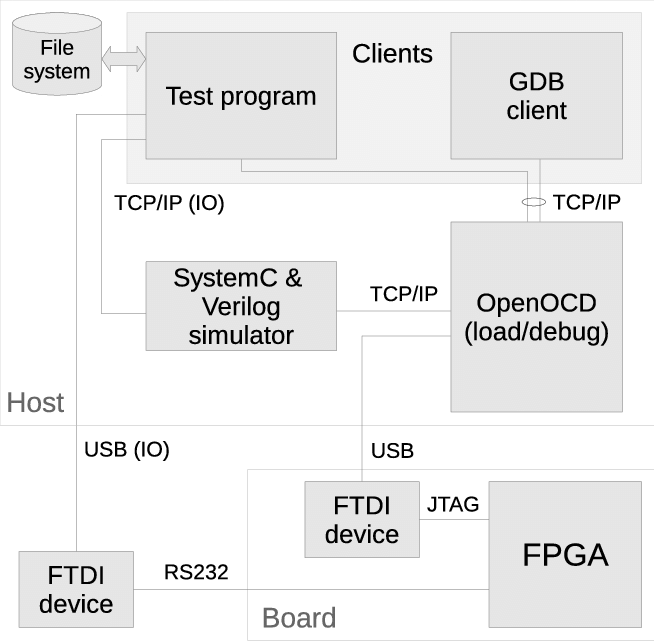
\includegraphics[width=0.5\linewidth]{Figures/env_warpbird}
	\caption{Warpbird's verification environment (figure taken from \cite{bib:warpbird}).}
	\label{fig:env_warpbird}
\end{figure}

Warpbird's verification environment is already described in \cite{bib:warpbird}, so this section will only refer and briefly detail some of its parts which contrast with the verification environment envisioned for \socname, so to emphasize the novelties introduced in respect to Warpbird.

Warpbird uses a JTAG tap which communicates with the host computer via an FTDI bridging device that translates JTAG to USB and vice-versa. The USB side of the FTDI devide then connect to OpecnOCD~\cite{bib:openocd}, an universal chip debug tool that provides a unified target access mechanism, facilitating the implementation of the communication structure between clients (such as the test program and GDB) and the FPGA.

OpenOCD allows debugging of programs running remotely on the FPGA using GDB, as if those programs were being ran locally. A test program is connected via a TCP/IP socket internal to the host machine to send OpenOCD commands such as program loading, execution halt and start, etc to the FPGA. OpenOCD is also connected via an internal TCP/IP socket to Verilator~\cite{bib:verilator} (SystemC \& Verilog simulator) to allow debugging on the RTL simulation target as well.

\subsection{\socname verification environment}
The verification environment for \socname will be based on Warpbird's. However, some adaptations must be made because the toolchains are different in the two and the two SoCs do not have the same interfaces to communicate with the outside world. For example, unlike Warpbird, \socname does not use the Rocket Chip generator and Chisel3 scala embedded language tools and has an Ethernet interface instead of a JTAG tap, which Warpbird has.

Because the JTAG tap is not used in \socname, we no longer need to use OpenOCD and the FT4232H Mini Module, which was used to bridge communications from the host machine to the JTAG pins in the FPGA board, which in turn were connected to Warpbird's JTAG tap, inside the FPGA itself. The FT2232H device\footnote{i.e. the FTDI device in the lower left corner in Figure~\ref{fig:env_warpbird}} is no longer necessary as well, because the Ethernet interface in \socname allows the clients (i.e. the test program and GDB) can communicate with the FPGA via Ethernet instead of converting USB streams from the host computer into RS232 streams to the FPGA and vice-versa.

\begin{figure}[!h]
	\centering
	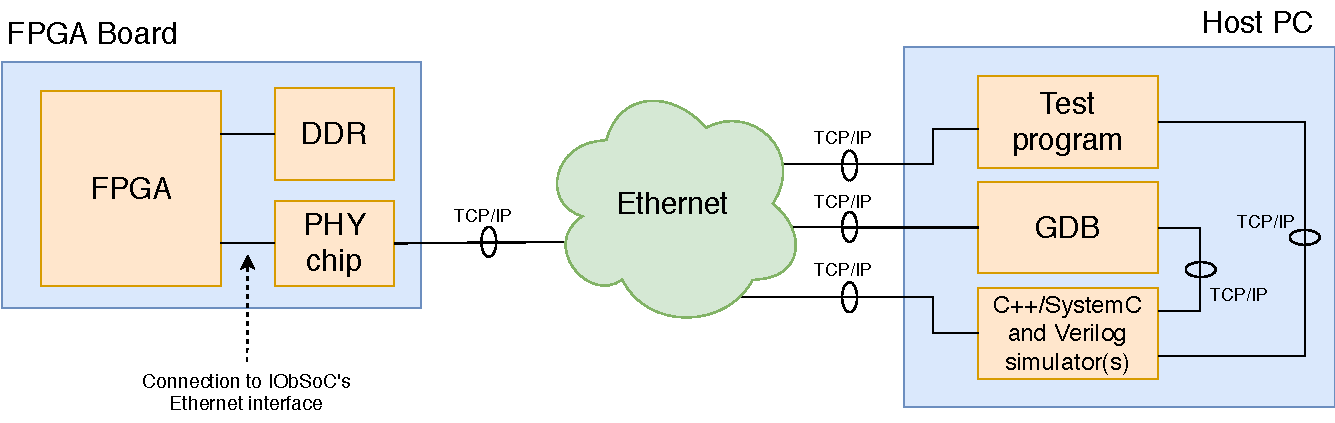
\includegraphics[width=1\linewidth]{Figures/env}
	\caption{Verification environment based on \socname.}
	\label{fig:env}
\end{figure}

Therefore, all communications between the host computer and the FPGA are now done using Ethernet, which simplifies the verification environment structure, as it can be seen in Figure~\ref{fig:env} compared to Figure~\ref{fig:env_warpbird}. On top of that, Ethernet is the most popular link-layer protocol on which TCP/IP is carried out, so this Ethernet communication infrastructure is an appealing choice. Because OpenOCD no longer exists in the verification environment, the C++/SystemC and Verilog simulator(s), the test program and the GDB client communicate directly with the FPGA via a TPC/IP socket which runs on top of an Ethernet connection. Also, GDB's communication with the simulator(s) is now done via a direct internal TCP/IP socket in the host machine, just like the one that already exists between the test program and the simulator(s).

The use of this new Ethernet infrastructure not only simplifies the verification environment but also makes communications between the host machine and the FPGA (or the SoC) much faster, because Ethernet bandwidth ranges between 10 Mbit/s and 100 Gbit/s, when JTAG's typical maximum bandwidth is several tens of Mhz. Besides this new way of communication between the host PC and the FPGA, most of the remaining structure of the verification environment will be similar to Warpbird's. 

After peripherals are added to \socname, SoC verification begins with RTL simulation, where dedicated testbenches and test programs are produced to test and evaluate it (these topics are better described in Section~\ref{section:devel_flow}). The simulators considered to integrate this environment are:

\begin{itemize}
	\item \textbf{Verilator}~\cite{bib:verilator}, which converts the Verilog description the SoC design to a C++/SystemC equivalent cycle-accurate behavioral model. This allows fast simulation of complex and large systems, but limits the truth values to 0 and 1, whereas other simulators use Z (high impedance), U (undefined) and others. Verilator is free and open source;
	
	\item \textbf{Icarus Verilog}, which is an open source simulation and synthesis tool more suited for small or medium-small sized projects. For medium to large-sized projects, a proprietary simulator or Verilator are better options, as Icarus becomes too slow, which may lead to project delays;
	
	% UM DOS OBJETIVOS É QUE O AMBIENTE DE DESENVOLVIMENTO SEJA OPEN SOURCE, POR ISSO NÃO SEI SE O NCSIM DEVE SER REFERIDO OU NÃO.
	\item \textbf{NCsim}, a commercial proprietary simulation engine contained in Cadence's design and verification tools suite. Although proprietary and very expensive, such a simulation tool may sometimes be necessary for large projects to be completed in a reasonable time window. Instituto Superior T\'{e}cnico makes NCSim available in machines that can be remotely accessed by students, professors and researchers at the university. The licenses for NCSim are payed with the help on European Union (EU) funds.
\end{itemize}

The waveforms generated by the simulations are then viewed in a waveform viewer such as GTKWave (a free waveform viewer). If errors are encountered, the SoC design must be rectified and new RTL simulations need to be made. After obtaining the expected results, the second step of the verification process is to target an FPGA and implement the SoC. When a bitstream is successfully generated, deployment of the SoC in the FPGA is made and tests are made in the FPGA emulated SoC. Every time unexpected problems occur, the verification needs to take a step back to the previous phases until all problems are solved. In each development stage that uses the verification environment\footnote{As it will be described in Section~\ref{section:devel_flow}, all development stages except in the first one, which is the toolchain installation.}, after successfully deploying the SoC in the FPGA, development advances to the next stage.

Another detail to account for is that because \socname does not have a debug module (unlike Warpbird), it is necessary to develop software to implement useful (and some indispensable) debug commands such as break, run, halt, continue, peek and poke. This debug program will be stored in the external DDR memory.


%%%%%%%%%%%%%%%%%%%%%%%%%%%%%%%%%%%%%%%%%%%%%%%%%%%%%%%%%%%%%%%%%%%%%%%%

\section{Development flow}
\label{section:devel_flow}
The development flow in which the SoC development environment will be based is the same as the one used in \cite{bib:blackbird,bib:warpbird}, which is illustrated in Figure~\ref{fig:devflow}.

\begin{figure}[!h]
	\centering
	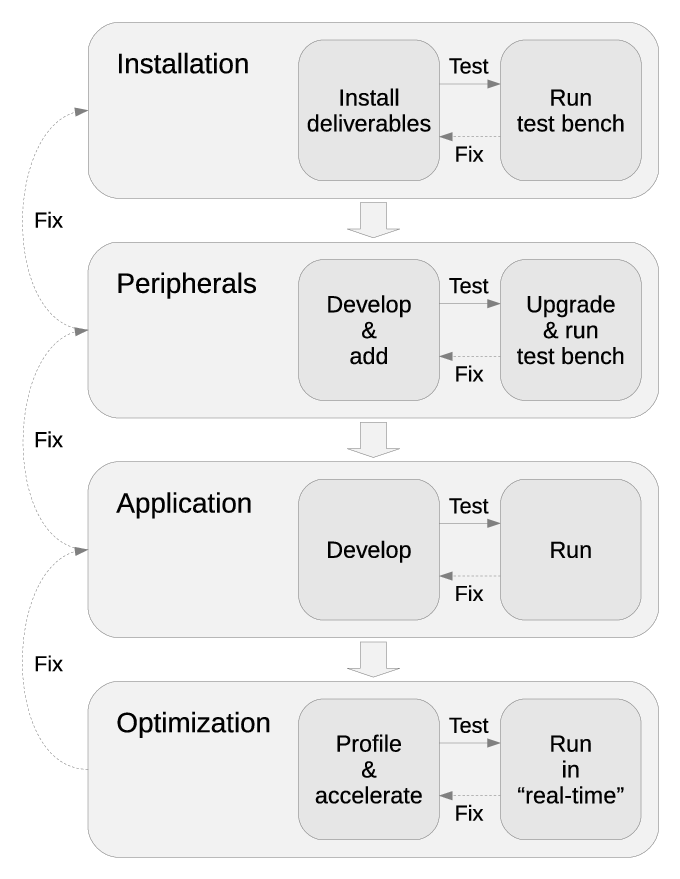
\includegraphics[width=0.5\linewidth]{Figures/devflow}
	\caption{Development flow (figure taken from \cite{bib:blackbird}).}
	\label{fig:devflow}
\end{figure}

\subsection{Toolchain installation}

%referir que as makefiles do picorv32 permitem instalar rapidamente o subconjunto necessario da toolchain do risc-v para que os testbenches básicos %corram sem problemas. Instala outras coisas, ver melhor o que (talvez o verilator?)
%listar algumas coisas to toolchain do risc-v que são instaladas para o picorv
%fazer uma lista de todas as ferramentas instaladas

The first stage of the development flow is the installation of the tools necessary to develop the SoC, such as compiler, assemblers, linkers, simulators and others. The PicoRV32's GitHub repository~\cite{bib:picorv32} provides a Makefile script to install the complete RISC-V toolchain. However, it is not necessary to install all of its tools, as some are not used by PicoRV32. 

The default settings of the build scripts available in the riscv-tools repository~\cite{bib:riscvtools} build a compiler, assembler and linker that can target any RISC-V ISA. However, the libraries are built for RV32G and RV64G targets. For this reason, the README file in PicoRV32's GitHub repository~\cite{bib:picorv32} also provides instructions with Linux shell and make commands to install a pure RV32I, RV32IC, RV32IM or RV32IMC CPU (including libraries). These commands include:

\begin{enumerate}
	\item the installation of various software packages\footnote{The list of packages installed can be seen in the shell commands provided in \cite{bib:picorv32}, in the \textit{Building a pure RV32I Toolchain} topic.};
	\item the creation of the installation directory inside the /opt folder;
	\item the download of the RISC-V GNU toolchain from \cite{bib:riscvgnutools} using git commands;
	\item building the toolchain in the host machine with a configure script.
\end{enumerate}

After installing the toolchain, a testbench is ran with standard configurations to check if the former was correctly installed. The testbench uses the Icarus Verilog simulation and synthesis tool ~\cite{bib:icarus}. There is also a simpler testbench that does not require an external firmware .hex file, which can be useful in systems that do not have the RISC-V compiler toolchain installed.

\subsection{Adding peripherals to \socname}
In the second stage of development, SoC components are added to \socname by describing them with the Verilog HDL. The example projects' files provided in PicoRV32's GitHub repository \cite{bib:picorv32} can provide helpful guidelines for this task. The peripherals to be added can be used as co-processors using PicoRV32's Pico Co-Processor Interface (PCPI) or can simply be connected to a PicoRV32 core through the AXI4-Lite memory interface provided. More PicoRV32 cores can be instantiated and interconnected using its native memory interface.

The standard RISC-V ISA extensions supported by PicoV32 can be added by turning on Verilog \textit{`define} flags in PicoRV32's Verilog description file (picorv32.v). When used, the multiply core provided in the repository in connected to PicoRV32 through the PCPI interface. One must remember to active the PCPI interface enable flag for the multiply core to work.

% ACHO QUE NÃO DOMINO SUFICIENTEMENTE BEM ESTES PORMENORES PARA FALAR BEM DELES...
% When new hardware or software components are added, the cross-compiler needs to become aware of the new hardware. There are options to make the compilation aware of new hardware units.

The verification environment described in Section~\ref{section:verification_env} is used to test the new SoC components. After being sure the peripherals are correctly connected and working, the SoC development may advance to the next stage.

\subsection{Application development}
Next, the software application to be ran in the SoC's CPU is developed using an IDE. Since no IDE integration is provided, the IDE can be chosen by the company or developer. The application can be ran in the verilated model of the SoC (i.e., the equivalent C++/SystemC model obtained with Verilator), generating cycle-accurate results, and in the FPGA emulated SoC, which is faster and more accurate. Debugging the application in both targets using GDB is also possible. These features are already detailed in Section~\ref{section:verification_env}.

The verification environment is once again used in this development stage in order to test the software application. After assuring the software implements the desired functionality, development advances to the final stage.

\subsection{Optimization}
The final development stage consists on optimizing the application developed in the previous stage. In order optimize software applications, profilers are used. A profiler is a dynamic program analysis tool that measures, for example, the frequency and duration of each function call in a program, the usage of instructions (i.e., the total number of times an instruction is used) and the memory space and time complexities of a program. This allow the software developer to understand which aspects or code blocks are affecting performance the most, identifying more easily the software components that should be priorly optimized.

The RISC-V toolchain does not have a profiler available. A way to work around this issue in software development using C or C++ is to use timing libraries such as time.h or other more appropriate ones to a targeted FPGA board to measure the time duration of each function call. Furthermore, for easing the use of this feature, one can use the pre-build compiler directives to turn the time measure feature on and off by simply uncommenting or commenting a compiler flag definition. An example is provided in the following piece of C code:
\begin{lstlisting}[frame=single,basicstyle=\footnotesize\ttfamily,linewidth=\columnwidth,breaklines=true,language=C]
#define COUNT_TIME // comment/uncomment this line to shut off/on time measure feature

// more code

#ifdef COUNT_TIME
start_time_count_routine();  // assume time duration value's mem. space is selected here
#endif
some_function_call();
#ifdef COUNT_TIME
finish_time_count_routine(); // assume time duration value is stored here 
#endif

// more code
\end{lstlisting}